\documentclass{article}

\author{Teddy Krulewich}
\title{\vspace{-4em}HW2 ME5501 – Robotics and Unmanned Systems}

\usepackage[utf8]{inputenc}
\usepackage{minted}
\usepackage{hyperref}
\usepackage{xcolor}
\definecolor{bg}{rgb}{0.95,0.95,0.95}
\usepackage{caption}
\usepackage{mdframed}

\usepackage{graphicx}
\graphicspath{ {images/} }

\begin{document}
\maketitle

\noindent All code may be found at: \url{https://github.com/tkrulewich/teddy_krulewich_unmanned_systems/tree/main/teddy_krulewich_unmanned_systems/week_2}

\section*{Problem 1}

Create a function that checks if the current node is valid based upon the list of obstacles, grid 
boundaries, and current location. 
Using an obstacle list of (1,1), (4,4), (3,4), (5,0), (5,1), (0,7), (1,7), (2,7), and (3,7); and a bounding box 
of 0 to 10 for both x and y, and step size of 0.5, verify that the location (2,2) is valid. Assume the 
obstacles have a diameter of 0.5 (only occupy the node at which they reside).
Pass the obstacle list, node, and map boundaries/step size, and return a Boolean True/False 
depending on if the node location is valid (reachable).
Submit your Python code

\bigskip
I chose to invalid nodes in c-space when they are added to the grid using a bounding box system.
This is more efficient as we dont have to check the entire space for invalid nodes and adding obstacles
doesnt path finding time. The code is below:
\bigskip
\begin{mdframed}[backgroundcolor=bg]
\begin{minted}{python}
def node_valid(self, node: Node) -> bool:
  """Returns true if the given node is valid. 
  Meaning it is within the grid bounds and does 
  not collide with any obstacles"""

  return (node in self.valid_nodes and 
      self.bounds.contains_node(node))


def add_obstacle(self, obstacle: Obstacle) -> None:
  """Adds an obstacle to the grid and invalidates all nodes 
  that collide with it"""
  self.obstacles.append(obstacle)
  self.invalidate_neighboring_nodes(obstacle)

def invalidate_neighboring_nodes(self, obstacle: Obstacle):
  """Invalidates all nodes that collide with an obstacle"""

  # get the obstalce bounding box
  bounds = obstacle.get_bounding_box()

  # round the obtacle bounding box to the grid spacing
  bounds.min_x = self.spacing * 
      math.floor(bounds.min_x / self.spacing)
  bounds.max_x = self.spacing * 
      math.ceil(bounds.max_x / self.spacing)

  bounds.min_y = self.spacing * 
    math.floor(bounds.min_y / self.spacing)
  bounds.max_y = self.spacing *
    math.ceil(bounds.max_y / self.spacing)

  # invalidate all nodes that are within the bounding box
  for y in np.arange(bounds.min_y, 
      bounds.max_y + self.spacing, 
      self.spacing):
    
    for x in np.arange(bounds.min_x, 
        bounds.max_x + self.spacing, 
        self.spacing):
      if (x, y) in self.nodes:

        node = self.get_node(x, y)
        if (node in self.valid_nodes 
          and obstacle.collides_with(node)):

          self.valid_nodes.remove(node)

\end{minted}
\end{mdframed}

\begin{mdframed}[backgroundcolor=bg]
\begin{minted}{python}
grid = Grid(0, 10, 0, 10, 0.5)

grid.add_obstacles([
  Obstacle(1,1, 0.25),
  Obstacle(4,4, 0.25),
  Obstacle(3,4, 0.25),
  Obstacle(5,0, 0.25),
  Obstacle(5,1, 0.25),
  Obstacle(0,7, 0.25),
  Obstacle(1,7, 0.25),
  Obstacle(2,7, 0.25),
  Obstacle(3,7, 0.25)
])

print(grid.node_valid(grid.get_node(2,2)))
\end{minted}
\end{mdframed}
\noindent\rule{\textwidth}{0.4pt}\\
\textbf{Output: True}


\section*{Problem 2}


\textbf{See pseudocode on Canvas for significant assistance in the implementation of Dijkstra’s 
Algorithm.}

\bigskip
Integrate your functions into a script with a function that runs Dijkstra’s algorithm given the starting 
location, goal location, grid information, and obstacle list. The function should end with a plot 
showing the grid space with obstacles (can just use markers for the obstacles) and the desired path 
from the start location to the goal location. Your function should return this list of waypoints for the 
desired path. The waypoint list will be used for the Turtlebots later in the semester.
Use the grid information above (Problem 1) with a starting location of (0,0) and a goal location of (8,
9). 
Show the plot of the grid and desired path.
Submit your Python code.

\begin{figure}[h]
    \centering
    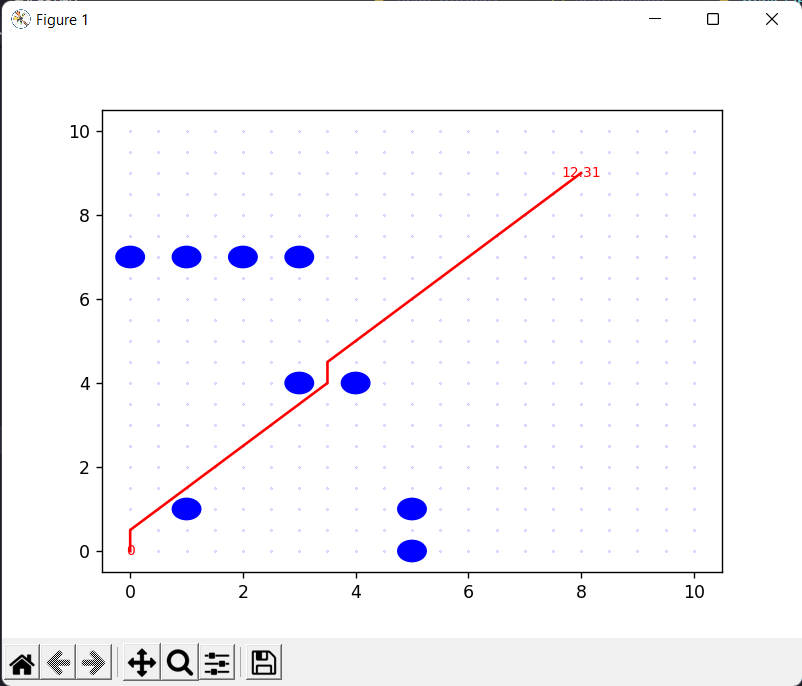
\includegraphics[width=12cm]{question2.png}
    \caption*{Shortest Path from (0,0) to (8,9)}
\end{figure}

\bigskip
\begin{mdframed}[backgroundcolor=bg]
\begin{minted}{python}
def dijkstras(self, start, end) -> tuple[list[float], list[float]]:
  """Finds the shortest path using Dijkstra's algorithm"""
  start.cost = 0

  current_node : Node = start

  unvisited = set(self.nodes.values())

  # to reduce search space we only consider nodes
  #  that we have "seen" before
  seen = set([current_node])
  visited = set()

  # loop through unvisited nodes
  while len(unvisited) > 0:
    unvisited.remove(current_node)
    visited.add(current_node)
    
    # get the possible neighbors of the current node
    for y in np.arange(current_node.y - self.spacing, 
      current_node.y + 2 * self.spacing, self.spacing):

      for x in np.arange(current_node.x - self.spacing,
        current_node.x + 2 * self.spacing, self.spacing):

        # if there is a neighbor node at that coordinate
        if ((x, y) in self.nodes):
          neighbor = self.nodes[(x,y)]
          if (neighbor is not current_node
             and neighbor not in visited
             and self.node_valid(neighbor)):
            # add it to the list of seen nodes
            seen.add(neighbor)

            # update the cost if its less than previous cost
            cost = (current_node.cost
                 + current_node.distance(neighbor))
            if (cost < neighbor.cost):
              neighbor.cost = cost
              neighbor.parent_node = current_node
              
    # if there are more unvisited nodes
    # visit the next one with lowest cost
    if len(unvisited) > 0:
      seen.remove(current_node)
      if (len(seen) == 0):
        break
      current_node = min(seen, key=lambda x: x.cost)
    
  
  # store x and y coordinates of nodes in path for plotting
  x_list = []
  y_list = []

  # start from the end node and work backwars to the start
  current_node = end
  while current_node != None:
    x_list.append(current_node.x)
    y_list.append(current_node.y)

    current_node = current_node.parent_node
  
  # plot cost of start and end
  plt.text(start.x, start.y, str(round(start.cost, 2)), 
    color="red", fontsize=8, horizontalalignment="center", 
    verticalalignment = "center")

  plt.text(end.x, end.y, str(round(end.cost, 2)), 
    color="red", fontsize=8, horizontalalignment="center", 
    verticalalignment = "center")

  return x_list, y_list
\end{minted}  
\end{mdframed}

\section*{Problem 3}

Problem 3 (10 pts):
Assuming the robot has an actual size, you will need to inflate the graph such that the algorithm does 
not plan such that it would contact the robot. Use a robot diameter of 1.0. This inflation can occur in 
several different methods including: 1) inflate the obstacle list and grid boundary, 2) when checking 
for a collision between a node and the grid boundary or obstacle, see if the distance to the obstacle is 
less than the robot diameter (rather than checking for distance = 0).

\bigskip
\noindent Rerun the same grid/configuration used for Problem 2 and show the results


\bigskip
After inflating the graph for a robot of diamater 1, the path from (0,0) to (8,9) is no longer valid.
Instead I have shown the path from (2,2) to (8,9) with the inflated graph.

\begin{figure}[h]
    \centering
    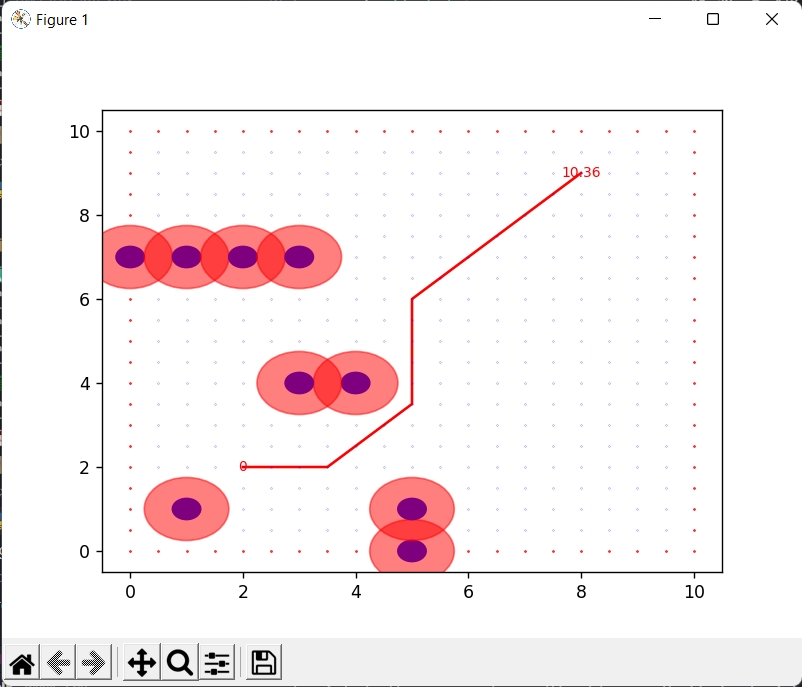
\includegraphics[width=12cm]{question3.png}
    \caption*{Shortest Path from (2,2) to (8,9) with inflation}
\end{figure}


\end{document}